\chapter{Projekt aplikacji mikroserwisowej}
\section{Założenia aplikacji}
\par Budowany projekt aplikacji z założenia ma symulować podstawowe funkcjonalności internetowej księgarni. Cały system został rozbity na niewielkie usługi z których każda wykonuje ściśle określone działanie w swojej domenie. Poniżej znajduje się lista dostępnych działań przewidzianych dla użytkownika. 
\begin{itemize}
    \item Utworzenie konta użytkownika korzystającego z sklepu,
    \item Dodanie książki do magazynu,
    \item Utworzenie zamówienia,
    \item Pobranie listy wszystkich zamówień dla danego użytkownika,
    \item Pobranie dostępnych książek znajdujących się w magazynie,
    \item Pobranie konkretnej pozycji z katalogu podając numer identyfikacyjny książki,
    \item Pobranie listy użytkowników posiadających konto wraz za datami utworzenia konta,
\end{itemize}
\section{Diagram przypadków użycia}
\par Diagram przedstawiony na rys. 4.1 przedstawia wszystkie możliwe czynności możliwe do wykonania przez system. Dwa przypadki stanowią bazę dla  W tym przypadku usługa zamówienia wykorzystując usługi świadczone przez pozostałe mikroserwisy może wymieniać się potrzebnymi danymi nie mając dostępu do bazy danych, gdzie są przechowywane.
\begin{figure}[h]
    \caption{Diagram przypadków użycia}
    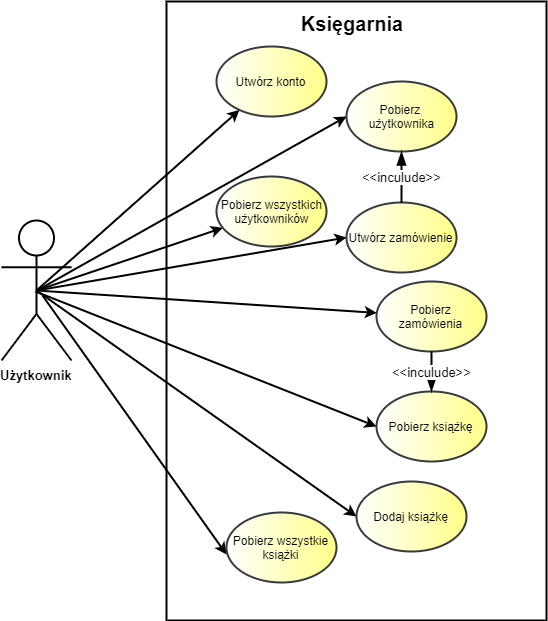
\includegraphics[width=\textwidth]{use_case}
    \centering
\end{figure}
\newpage
\section{Schemat blokowy systemu}
\par System opiera się na współpracujących ze sobą usługach sieciowych. Każda z tych usług działa niezależnie od reszty dzięki temu wdrożenie nowej wersji nie powoduje przerwania w działaniu innej. Dobra praktyka przy projektowaniu usług mikroserwisowych zaleca, aby każdy serwis korzystał z niezależnej bazy danych. Projekt uwzględnia i to podejście. Użytkownik do komunikowania z usługami będzie używał API, które będzie wystawiało wszystkie potrzebne metody na zewnątrz do użytku publicznego. Schemat poszczególnych modułów oraz powiązań został przedstawiony na rys. 4.2 
\begin{figure}
    \caption{Diagram przedstawiający architekturę aplikacji}
    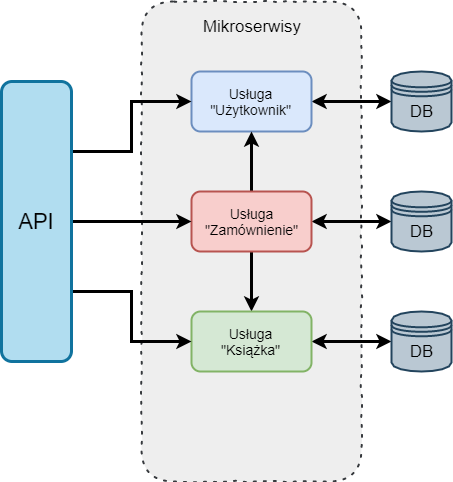
\includegraphics[width=\textwidth]{microservices_diagram_block}
    \centering
\end{figure}